% Time-stamp: <2025-02-27 04:07:34 amano>

% main file
\documentclass[luatex,twocolumn,showpacs,aps,prb,reprint,amsfonts,amsmath,amssymb,floatfix,groupedaddress, longbibliography]{revtex4-2} 
% preamble 
% preamble

% This is for template only !!
\usepackage{lipsum}

%\usepackage{floatrow}
\usepackage{siunitx}
\usepackage{color}
\usepackage{hhline}
\usepackage{mathrsfs}
\usepackage[dvipdfmx]{graphicx}
\usepackage{adjustbox}
\usepackage{dcolumn}
\usepackage{bm}% bold math
\usepackage{multirow}
\usepackage{booktabs}
\usepackage{afterpage}
\usepackage{amsmath}
\usepackage{ulem}
\usepackage{physics}

% https://mathlandscape.com/latex-underline/
\usepackage{ulem}

\usepackage{here} % force figures Here.

\usepackage[inline]{asymptote}

\usepackage[compat=1.1.0]{tikz-feynhand} % feynman diagram
% subcaption http://www.yamamo10.jp/yamamoto/comp/latex/make_doc/insert_fig/index.php#SUBCAP
% https://oku.edu.mie-u.ac.jp/tex/mod/forum/discuss.php?d=1024
% https://atatat.hatenablog.com/entry/cloud_latex18_subcaption
\usepackage{caption}
\usepackage[subrefformat=parens]{subcaption}
%\usepackage{floatrow}
%\usepackage[export]{adjustbox}

% http://www.yamamo10.jp/yamamoto/comp/latex/make_doc/chemistry/index.php
\usepackage[version=4]{mhchem}

% for tikz 
\usepackage{tikz, pgf, pgfplots, pgfplotstable}
\usepackage{tikz-3dplot}
\usetikzlibrary{math,calc}
\pgfplotsset{compat = newest}
\usepgfplotslibrary{groupplots} % LATEX and plain TEX
\pgfplotsset{compat = newest}

\pgfplotsset{
   table/search path={figures/self_energy, figures/tdos, figures/diel_func, figures/band},
}

\graphicspath{{figures/self_energy, figures/tdos, figures/diel_func, figures/band}}

% https://tikz.dev/library-external
% crisさんおすすめ
% \usetikzlibrary{external}
% \tikzexternalize % activate!

\usepackage{multirow}

\usepackage[nohyperlinks,nolist]{acronym} % abbreviation

\usepackage[subpreambles=true,sort=true]{standalone}

%https://uec.medit.link/latex/table.html#:~:text=%E3%82%BB%E3%83%AB%E3%81%AE%E7%B5%90%E5%90%88,%E3%82%92%E8%AA%AD%E3%81%BF%E8%BE%BC%E3%82%80%E5%BF%85%E8%A6%81%E3%81%8C%E3%81%82%E3%82%8B%E3%80%82

% \usepackage[no-math,haranoaji,deluxe]{luatexja-preset}
%https://mizunashi-mana.github.io/blog/posts/2021/12/migrate-to-luatexja/

\newcommand{\red}[1]{\textcolor{red}{#1}}
\newcommand{\blue}[1]{\textcolor{blue}{#1}}
\arraycolsep=0.0em
\setlength{\abovecaptionskip}{0mm}
\setlength{\belowcaptionskip}{0mm}
\usepackage{caption} 
\captionsetup[table]{skip=8pt}
\captionsetup[figure]{skip=4pt}
%\setlength{\MidlineHeight}{2pt}


\usepackage{comment}
%\usepackage{natbib}

\usepackage[colorlinks=true,citecolor=blue,linkcolor=blue,urlcolor=blue]{hyperref}
\usepackage{cleveref}
\crefname{equation}{Eq.}{Eq.}% {環境名}{単数形}{複数形} \crefで引くときの表示
\crefname{figure}{Fig.}{Fig.}% {環境名}{単数形}{複数形} \crefで引くときの表示
\crefname{table}{Table}{Table}% {環境名}{単数形}{複数形} \crefで引くときの表示
\crefname{section}{Sec.}{Sec.}% {環境名}{単数形}{複数形} \crefで引くときの表示
\crefname{appendix}{Appendix}{Appendix}% {環境名}{単数形}{複数形} \Crefで引くときの表示


\Crefname{equation}{Equation}{Equation}% {環境名}{単数形}{複数形} \Crefで引くときの表示
\Crefname{figure}{Figure}{Figure}% {環境名}{単数形}{複数形} \Crefで引くときの表示
\Crefname{table}{Table}{Table}% {環境名}{単数形}{複数形} \Crefで引くときの表示
\Crefname{section}{Section}{Section}% {環境名}{単数形}{複数形} \Crefで引くときの表示
\Crefname{appendix}{Appendix}{Appendix}% {環境名}{単数形}{複数形} \Crefで引くときの表示



\usepackage{threeparttable} %https://qiita.com/kumamupooh/items/38795811fc6b934a950d
% bookmark
% \usepackage{xurl}
% \hypersetup{unicode,bookmarksnumbered=true,hidelinks,final}


\newcommand{\ph}{\phantom{0}}

\renewcommand{\topfraction}{1.0}
\renewcommand{\bottomfraction}{1.0}
\renewcommand{\dbltopfraction}{1.0}
\renewcommand{\textfraction}{0.1}
\renewcommand{\floatpagefraction}{0.9}
\renewcommand{\dblfloatpagefraction}{0.9}



% path setting
% ======================
%  ファイルを分割した時のpath設定 
% figure(pgfplot), graphics, input
%


\pgfplotsset{
   table/search path={figures/self_energy, figures/tdos, figures/diel_func, figures/band},
}

\graphicspath{{figures/self_energy, figures/tdos, figures/diel_func, figures/band}}

% https://scrapbox.io/hada/LaTeX%E3%82%BD%E3%83%BC%E3%82%B9%E3%81%AEinput_path
 \makeatletter
 \providecommand*{\input@path}{}
 \g@addto@macro\input@path{{docs/}{include/}}% append
 \makeatother

\begin{document}

\title{HOGEHOGE \\
FUGAGUGA}

\author{HOGE HOGE$^{1}$ }
\author{FUGA FOGE$^{2}$ }
\author{HOGE HOGE$^{1,3}$ }
\affiliation{$^1$HOGEHOGE}
\affiliation{$^2$FUGAGUFA}
\affiliation{$^3$HOGEHOGE}
\affiliation{$^4$FUGAGUFA}

\date{\today}


\onecolumngrid

\begin{abstract}
 \lipsum[1-1]
\end{abstract}

\twocolumngrid


\maketitle



 % https://ramibaddour.com/2017/01/18/latex-working-with-acronyms/
 % \renewcommand{\baselinestretch}{10.0}
 \begin{acronym}[PPG725]
 % https://tex.stackexchange.com/questions/95640/acronyms-list-size
 %  \setlength{\parskip}{0ex}
  \setlength{\itemsep}{4.0pt}
     \acro  {H-bond}[H-bond] {hydrogen bond} 
     \acrodefplural{H-bond}[H-bonds] {hydrogen bonds} % https://tex.stackexchange.com/questions/38558/how-to-pluralize-an-acronym-which-ends-in-s-correctly
     \acro  {DPMD}  [DPMD]   {deep potential molecular dynamics}
     \acro  {RMSE}  [RMSE]   {root mean square error}
     \acro  {RDF}   [RDF]    {radial distribution function}
     \acro  {KS}    [KS]    {Kohn-Sham} % finish
     \acro  {O-lp}  [O-lp]  {O lone-pair} % finish
     \acro  {DFPT}  [DFPT]  {density functional perturbation theory} % finish
     \acro  {DFT}   [DFT]   {density functional theory}
     \acro  {ML}    [ML]    {machine learning}
     \acro  {VACF}  [VACF]  {velocity auto-correlation function}
     \acro  {VDOS}  [VDOS]  {vibrational density of states}
     \acro  {PG}    [PG]    {propylene glycol}
     \acro  {PG2}   [PG2]   {di-propylene glycol}
     \acro  {PPG}   [PPG]   {polypropylene glycol}
     \acro  {PPG725}[PPG725]{14-mer of Propylene glycol }
     \acro  {WF}    [WF]    {Wannier function}
     \acro  {MLWF}  [MLWF]  {maximally-localized Wannier function}
     \acrodefplural{MLWF} [MLWFs]  {maximally-localized Wannier functions}
     \acro  {WC}    [WC]    {Wannier center}
     \acrodefplural{WC} [WCs]  {Wannier centers}
     \acro  {BC}    [BC]    {bond center}
     \acro  {CPMD}  [CPMD]  {Car-Parrinello molecular dynamics}
     \acro  {BOMD}  [BOMD]  {Born-Oppenheimer molecular dynamics}
     \acro  {CMD}   [CMD]  {classical molecular dynamics}
     \acro  {BO}    [BO]    {Born-Oppenheimer}
     \acro  {AIMD}  [AIMD]  {\textit{ab initio} molecular dynamics}
     \acro  {MD}    [MD]    {molecular dynamics}
     \acro  {lp}    [lp]    {lone-pair}   
     \acro  {THz}   [THz]    {terahertz}
     \acro  {IR}    [IR]     {infrared}

 %% Define a custom plural form of an acronym
 %    \acrodefplural{iot}[IoTs]{Internets-of-Things}
 %% Preferably, put all acronym definitions in one file and load it
 %   \input{acros.tex}
 \end{acronym}

% % intro
\section{Introduction}\label{sec:intro}

% dummy documents
\lipsum[1-10]

\begin{itemize}
 \item use ce command for chemical symbols
 \item space between letter and kakko
 \item for full paper, 5~6 danraku
 \item citation~\cite{abrahams1971Rutile} items are in references/
\end{itemize}


% figure
\begin{figure}[t]
%  \begin{minipage}[H]{0.45\linewidth}
%\captionsetup[subfigure]{font={bf,large}, skip=1pt, margin=-0.7cm,justification=raggedright, singlelinecheck=false}
\hfill
\centering
\begin{subcaptionblock}{0.6\linewidth}
\centering
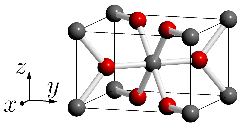
\includegraphics[]{rutile_axis-1_0.pdf}
\subcaption{}
\end{subcaptionblock}\hfill
\begin{subcaptionblock}{0.4\linewidth}
\centering
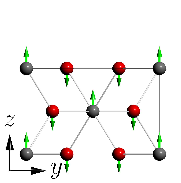
\includegraphics[width=\linewidth]{A2u.pdf}
\subcaption{$A_{\mathrm{2u}}$}
\end{subcaptionblock}\hfill
\begin{subcaptionblock}{0.3\linewidth}
\centering
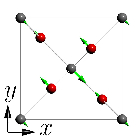
\includegraphics[width=\linewidth]{E1u.pdf}
\subcaption{$E^{1}_{\mathrm{u}}$}
\end{subcaptionblock}\hfill
\begin{subcaptionblock}{0.3\linewidth}
\centering
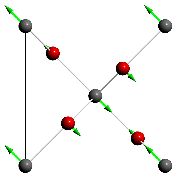
\includegraphics[width=\linewidth]{E2u.pdf}
\subcaption{$E^{2}_{\mathrm{u}}$}
\end{subcaptionblock}\hfill
\begin{subcaptionblock}{0.3\linewidth}
\centering
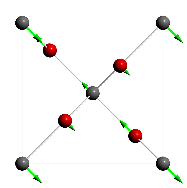
\includegraphics[width=\linewidth]{E3u.pdf}
\subcaption{$E^{3}_{\mathrm{u}}$}
\end{subcaptionblock}\hfill
% \subfloat[][]{%\label{fig:modes}
%\begin{tabular}[b]{@{}c@{}}
%\end{tabular}%
%}
\caption{(a) The unit cell of rutile \ce{TiO2}, which contains two titanium atoms (black) and four oxygen atoms (red). (b-e) Schematic views of atomic displacements for the $A_{\mathrm{2u}}$ mode and the three $E_{\mathrm{u}}$ modes. }
% BZありversion \caption{(a)The crystal structure of rutile \ce{TiO2}, (b) The first Brillouin zone and its high-symmetry points including $Z (0,0,0.5)$ (reduced coordinates), $A (0.5,0.5,0.5)$, $M (0.5,0.5,0)$, $R (0,0.5,0.5)$, and $X (0,0.5,0)$, and (c) schematic view of the A_{\mathrm{2u}} mode(left) and the Eu mode(right). }
\label{fig:crystal}
\end{figure}



% theory
\section{Theory}\label{sec:theory}

% dummy documents
\lipsum[1-10]




% result
\section{Results and Discussion}\label{sec:result}
\subsection{Result1}\label{subsec:result1}

% dummy documents
\lipsum[1-5]

% figure
\begin{figure}[t]
%  \begin{minipage}[H]{0.45\linewidth}
%\captionsetup[subfigure]{font={bf,large}, skip=1pt, margin=-0.7cm,justification=raggedright, singlelinecheck=false}
\hfill
\centering
\begin{subcaptionblock}{0.6\linewidth}
\centering
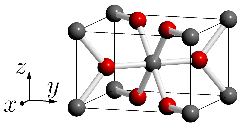
\includegraphics[]{rutile_axis-1_0.pdf}
\subcaption{}
\end{subcaptionblock}\hfill
\begin{subcaptionblock}{0.4\linewidth}
\centering
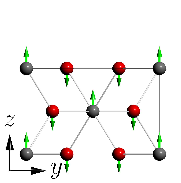
\includegraphics[width=\linewidth]{A2u.pdf}
\subcaption{$A_{\mathrm{2u}}$}
\end{subcaptionblock}\hfill
\begin{subcaptionblock}{0.3\linewidth}
\centering
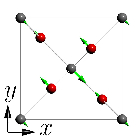
\includegraphics[width=\linewidth]{E1u.pdf}
\subcaption{$E^{1}_{\mathrm{u}}$}
\end{subcaptionblock}\hfill
\begin{subcaptionblock}{0.3\linewidth}
\centering
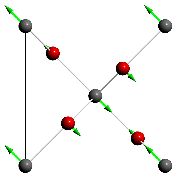
\includegraphics[width=\linewidth]{E2u.pdf}
\subcaption{$E^{2}_{\mathrm{u}}$}
\end{subcaptionblock}\hfill
\begin{subcaptionblock}{0.3\linewidth}
\centering
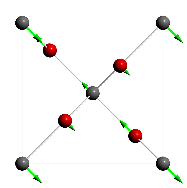
\includegraphics[width=\linewidth]{E3u.pdf}
\subcaption{$E^{3}_{\mathrm{u}}$}
\end{subcaptionblock}\hfill
% \subfloat[][]{%\label{fig:modes}
%\begin{tabular}[b]{@{}c@{}}
%\end{tabular}%
%}
\caption{(a) The unit cell of rutile \ce{TiO2}, which contains two titanium atoms (black) and four oxygen atoms (red). (b-e) Schematic views of atomic displacements for the $A_{\mathrm{2u}}$ mode and the three $E_{\mathrm{u}}$ modes. }
% BZありversion \caption{(a)The crystal structure of rutile \ce{TiO2}, (b) The first Brillouin zone and its high-symmetry points including $Z (0,0,0.5)$ (reduced coordinates), $A (0.5,0.5,0.5)$, $M (0.5,0.5,0)$, $R (0,0.5,0.5)$, and $X (0,0.5,0)$, and (c) schematic view of the A_{\mathrm{2u}} mode(left) and the Eu mode(right). }
\label{fig:crystal}
\end{figure}

% table

\begin{table}[tb] % RMSE [D]
\centering
\caption{RMSE $[\mathrm{D}]$ of \ac{ML} dipole models for \ac{PG} and PG2. The \ce{CO}, \ce{O}, and \ce{OH} models were trained for reference purposes and were not used for spectrum calculations. The CO+Olp+OH and CO+Olp+CO represents the COH and COC dipoles calculated from these three models, respectively.}
\includestandalone[mode=tex]{figures/table01/table01} %
\label{table:rmse}
\end{table}

\subsection{Result2}\label{subsec:result2}

% dummy documents
\lipsum[1-5]

% figure
\begin{figure}[t]
%  \begin{minipage}[H]{0.45\linewidth}
%\captionsetup[subfigure]{font={bf,large}, skip=1pt, margin=-0.7cm,justification=raggedright, singlelinecheck=false}
\hfill
\centering
\begin{subcaptionblock}{0.6\linewidth}
\centering
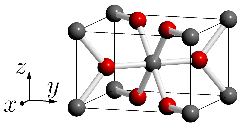
\includegraphics[]{rutile_axis-1_0.pdf}
\subcaption{}
\end{subcaptionblock}\hfill
\begin{subcaptionblock}{0.4\linewidth}
\centering
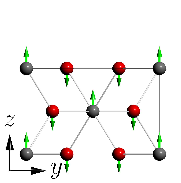
\includegraphics[width=\linewidth]{A2u.pdf}
\subcaption{$A_{\mathrm{2u}}$}
\end{subcaptionblock}\hfill
\begin{subcaptionblock}{0.3\linewidth}
\centering
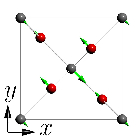
\includegraphics[width=\linewidth]{E1u.pdf}
\subcaption{$E^{1}_{\mathrm{u}}$}
\end{subcaptionblock}\hfill
\begin{subcaptionblock}{0.3\linewidth}
\centering
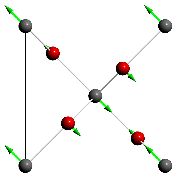
\includegraphics[width=\linewidth]{E2u.pdf}
\subcaption{$E^{2}_{\mathrm{u}}$}
\end{subcaptionblock}\hfill
\begin{subcaptionblock}{0.3\linewidth}
\centering
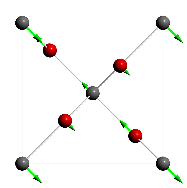
\includegraphics[width=\linewidth]{E3u.pdf}
\subcaption{$E^{3}_{\mathrm{u}}$}
\end{subcaptionblock}\hfill
% \subfloat[][]{%\label{fig:modes}
%\begin{tabular}[b]{@{}c@{}}
%\end{tabular}%
%}
\caption{(a) The unit cell of rutile \ce{TiO2}, which contains two titanium atoms (black) and four oxygen atoms (red). (b-e) Schematic views of atomic displacements for the $A_{\mathrm{2u}}$ mode and the three $E_{\mathrm{u}}$ modes. }
% BZありversion \caption{(a)The crystal structure of rutile \ce{TiO2}, (b) The first Brillouin zone and its high-symmetry points including $Z (0,0,0.5)$ (reduced coordinates), $A (0.5,0.5,0.5)$, $M (0.5,0.5,0)$, $R (0,0.5,0.5)$, and $X (0,0.5,0)$, and (c) schematic view of the A_{\mathrm{2u}} mode(left) and the Eu mode(right). }
\label{fig:crystal}
\end{figure}

% table

\begin{table}[tb] % RMSE [D]
\centering
\caption{RMSE $[\mathrm{D}]$ of \ac{ML} dipole models for \ac{PG} and PG2. The \ce{CO}, \ce{O}, and \ce{OH} models were trained for reference purposes and were not used for spectrum calculations. The CO+Olp+OH and CO+Olp+CO represents the COH and COC dipoles calculated from these three models, respectively.}
\includestandalone[mode=tex]{figures/table02/table02} 
\label{table:rmse}
\end{table}



\section{Conclusion}\label{sec:conclusion}

% dummy documents
\lipsum[2]




\begin{acknowledgments}
This research was funded by a HOMEHOME, FUGAGUGA and FUGAHUGA.
\end{acknowledgments}





\appendix

\section{Appendix1}\label{appendix:A}
% dummy documents
\lipsum[1-2]




% references
\bibliographystyle{apsrev4-2}
\bibliography{references/ref.bib}
\end{document}


% Local Variables:
% mode: yatex
% tex-main-file: t
% End: